\documentclass[10pt,a4paper,]{article}
%packages

\usepackage{fontawesome}

\usepackage{lmodern}
\usepackage[table,xcdraw]{xcolor}
\usepackage[T1]{fontenc}
\usepackage{tgpagella}
\usepackage[utf8]{inputenc}
\usepackage{algorithm}
\usepackage[noend]{algpseudocode}
\author{harry.filis}
\usepackage{multicol}
\usepackage{placeins}
\usepackage[utf8]{inputenc}
\usepackage[greek,english]{babel}
\usepackage{alphabeta}
\usepackage{csquotes}
\usepackage{amssymb}
\usepackage{amsmath}
\setlength{\headheight}{27.18134pt}
\usepackage{hyperref}
\usepackage[pdftex]{graphicx}
\usepackage{epstopdf}
\usepackage{blindtext}
\setlength{\columnseprule}{0.1pt}
\setlength{\columnsep}{3em}
\epstopdfsetup{update}
% \usepackage{subfigure}
\usepackage{float}
\usepackage{caption}
\usepackage{subcaption}
\usepackage{fancyhdr}
\usepackage{color}
\usepackage{xcolor}
\usepackage{listings}
\definecolor{softcyan}{RGB}{180,216,230}

\usepackage{listings}
\definecolor{codegreen}{rgb}{0,0.6,0}
\definecolor{codegray}{rgb}{0.5,0.5,0.5}
\definecolor{codepurple}{rgb}{0.58,0,0.82}
\definecolor{backcolour}{rgb}{0.95,0.95,0.92}
\usepackage{caption}
\DeclareCaptionFont{white}{\color{white}}
\DeclareCaptionFormat{listing}{\colorbox{gray}{\parbox{\textwidth}{#1#2#3}}}
\captionsetup[lstlisting]{format=listing,labelfont=white,textfont=white}
\lstset{
language=Python,
basicstyle=\tiny\ttfamily,
commentstyle=\ttfamily\color{gray},
numbers=left,
numberstyle=\ttfamily\color{gray}\tiny,
stepnumber=1,
numbersep=5pt,
backgroundcolor=\color{backcolour},
backgroundcolor=\color{white},
showspaces=false,
showstringspaces=false,
showtabs=false,
frame=single,
tabsize=2,
captionpos=!h,
breaklines=true,
breakatwhitespace=false,
label=\lstname,
escapeinside={},
keywordstyle={},
morekeywords={}
}
\DeclareCaptionFont{white}{\color{white}}
\DeclareCaptionFormat{listing}{\colorbox{gray}{\parbox{\textwidth}{#1#2#3}}}
\captionsetup[lstlisting]{format=listing,labelfont=white,textfont=white}

\DeclareMathOperator*{\argmin}{arg\,min}
%Title 
\pagestyle{fancy}
\fancyhf{}
\lhead{\texttt{SVM-CIFAR10}}
\rhead{\texttt{Φίλης Χάρης ΑΕΜ:9449}}
\chead{}
\lfoot{\texttt{$2^{η}$ Εργασία - {2022}}}
\cfoot{}
\rfoot{\texttt{Page \thepage}}
\renewcommand{\headrulewidth}{0.4pt}
\renewcommand{\footrulewidth}{0.4pt}
%links setup
\hypersetup{
    colorlinks=true,
    linkcolor=blue,
    filecolor=magenta,      
    urlcolor=codegreen,
}
\title{\texttt{\textlatin{Διναύσματα Μηχανικής Υποστήριξης για Διαχωρισμό Εικόνων σε Κλάσεις}} \\Support Vector Machines for Multiclass Classification - CIFAR10
\\
\begin{figure}[!htb]
    \centering
    \includegraphics[width = 6cm]{Decision-boundary-by-SVM-with-RBF-kernel-function.png}
    \label{linear_svm_classifier}%
\end{figure}
\newline
\texttt{Αριστοστέλειο Πανεπιστήμιο Θεσσαλονίκης \newline }
10ο Εξάμηνο ECE AUTh \\ 7o Εξάμηνο CSD AUTh \\ Νευρωνικά Δίκτυα - Βαθιά Μάθηση \\}
\author{\newline Χάρης Φίλης ΑΕΜ: 9449\\GitHub Repository Link : \href{https://github.com/ArtoriasAbyssslayer/DeepLearning-NNets}{\faGithubSquare} \\ GitHub Repository Folder : \href{https://github.com/ArtoriasAbyssslayer/DeepLearning-NNets/tree/master/SVM-Classification}{\faGithubSquare}
\\Update branch:\href{https://github.com/ArtoriasAbyssslayer/DeepLearning-NNets/tree/update_v2}{\faGithubSquare} }  
\date{December,2022}
\begin{document}
\maketitle
\newpage
   \bgroup
    \tableofcontents
    \let\clearpage\relax
    \listoffigures
    \egroup
\clearpage
\section{\texttt{Εισαγωγή}}
Αντικείμενο της παρούσας εργασίας, ήταν η συγγραφή ενός προγράμματος
που υλοποιεί ένα \textit{Support Vector Machine}(\textbf{SVM}), το οποίο επιλύει το πρόβλημα της κατηγοριοποίησης τριών κλάσεων. Το \textit{dataset} που επιλέχθηκε είναι το \textit{CIFAR10}, το οποίο έχει RGB εικόνες διάστασης 32x32\textit{px} και σκοπός των μοντέλων που δημιουργήθηκαν ήταν να διαχωρίσουν τις εικόνες σε όλες τις κλάσεις τους, αλλά αυτό το πείραμα που έτρεξε κυρίως(λόγω περιορισμένου χρόνου και υποχρεώσεων) είναι στο αρχείο \textit{svmCompare\_3ClassClassifier.py} και έχει κυρίως ως στόχο τον διαχωρισμό 3 κλάσεων του \textit{dataset} και συγκεκριμένα των κλάσεων \textit{σκύλος,γάτα,άλογο}. Παράλληλα έγινε επιλογή ενός πολύ μικρού υποσυνόλου \textit{training} 3000 δειγμάτων και για \textit{validation} 1000 δειγμάτων για να μην καθυστερήσει η εκπαίδευση αντιπροσωπευτικού set μοντέλων με γραμμικό ή \textit{rbf kernel}. Τέλος αξίζει να σημειωθεί πως δημιουργήθηκαν διάφορα μοντέλα όπως δύο \textit{from scratch SVM} το ένα που χρησιμοποιεί γραμμικό \textit{kernel} στο \textit{kernel trick} ενώ το άλλο \textit{rbf kernel}, ένα \textit{Linear SVM} που κάνει χρήση της βιβλιοθήκης \textit{LibLinear} της \textit{sklearn} και 3 μοντέλα που χρησιμοποιούν την \textit{\textit{LibSVM}} και το ένα από αυτά υλοποιεί \textit{PCA} ενώ το άλλο κάνει μετατοπίζει την λειτουργικότητα στο \textit{intel dataset}. Τέλος έγινε και ένα \textit{script} βελτιστοποίησης των υπερπαραμέτρων(\textit{model\_hyperparameter\_tunning.py}) των μοντέλων χρησιμοποιώντας την μέθοδο \textit{cross validation} για το ανακάτεμα και το σπάσιμο του \textit{dataset} και τον αλγόριθμο \textit{grid search} για την διερεύνηση βέλτιστων παραμέτρων. Δυστυχώς το μόνο που πρόλαβα να τρέξω(στα πλαίσια του χρόνου που είχα) ήταν το \textit{svmCompare} το οποίο υλοποιεί μοντέλα για διαχωρισμό 3 κλάσεων όπως ειπώθηκε. Ίσως στην παρουσίαση να έχω αποτελέσματα και από άλλα μοντέλα.
\section{Αλγόριθμος Κ πλησιέστερων γειτόνων}
Σαν προπαρασκευαστική εργασία είχαμε τρέξει το αλγόριθμο \textit{KNN} ο οποίος είναι ένας απλός σχετικά αλγόριθμος κατηγοριοποίησης δεδομένων με βάση το πόσο κοντά βρίσκονται τα δείγματα όσον αφορά την ευκλείδεια απόστασή τους. Ο συγκεκριμένος αλγόριθμος όπως είχαμε δείξει και σε προηγούμενες εργασίες δεν λειτουργεί με βάση να βελτιώνει αυτή την κατηγοριοποίηση που κάνει και πετυχαίνει αρκετά χαμηλά επίπεδα ακρίβειας στην κατηγοριοποίηση ενός σύνθετου \textit{dataset }εικόνων όπως είχαμε δείξει και βλέπουμε παρακάτω για πλήθος τριών γειτόνων. 
\begin{figure}[!htb]
    \centering
    \includegraphics[width=4cm]{Knn3.png}
    \caption{Classification report k=3}
    \label{fig:knn3}
\end{figure}
\newline
Αντίστοιχα και ίσως χειρότερα, είναι και τα αποτελέσματα του αλγορίθμου \textit{Nearest Class Centroid}, ο οποίος λειτουργεί με πιο απλή λογική συγκρίνοντας με ένα προεπιλεγμένο κέντρο νέα δείγματα
\begin{figure}[!htb]
    \centering
    \includegraphics[width=4cm]{NCC-results.png}
    \caption{Classification results nearest class centroids}
    \label{fig:knn3}
\end{figure}
\newline
Ωστόσο, όπως θα δούμε και στην συνέχεια επειδή τα μοντέλα που εκπαιδεύτηκαν με τον αλγόριθμο του \textit{SVM} δεν εκπαιδεύτηκαν σε μεγάλο σύνολο δεδομένων καθώς και επίσης ο ίδιος ο αλγόριθμος δεν αποτελεί \textit{state of art solution} στο πρόβλημα όπως τα \textit{MLP} που είδαμε ήδη τα αποτελέσματα που προέκυψαν είναι αρκετά απογοητευτικά σε επίπεδα που φτάνουμε και τις επιδόσεις του \textit{NCC}.Βέβαια όπως θα φανεί αργότερα, αν και ο \textit{K-NN} προσφέρει μεγαλύτερη ακρίβεια, δεν προσφέρει την βέλτιστη ταχύτητα για την πρόβλεψη νέων δεδομένων (μιας και είναι άπληστος αλγόριθμος) σε σχέση με  ένα \textit{SVM}. Η πολυπλοκότητα του \textit{KNN} είναι άμεσα εξαρτώμενη και μεγαλώνει όσο μεγαλώνει το training set. 

\section{Μηχανές Διανυσμάτων Υποστήριξης \textit{(SVM)}}
Για την κατασκευή των μηχανών διανυσμάτων υποστήριξης της εργασίας χρησιμοποιήθηκε τόσο η sklearn (το κομμάτι που χρησιμοποιεί την \textit{LibSVM} αλλά και το κομμάτι που λύνει το πρόβλημα στο \textit{\textbf{primal space}} \textit{LibLinear} με την διαμάχη των \textit{svm} με την τακτική one versus rest) όσο και \textit{from scratch προσπάθειες υλοποίησης}.
\subsection{Κατηγοριοποιητής τριών κλάσεων - \textit{3 class Support Vector Classifier(SVC)}}
Λόγων περιορισμένου χρόνου ο τύπος των κατηγοριοποιητών που εξετάστηκε είναι προϊόν της \textit{LibSVM} που χρησιμοποιεί η \textit{sklearn} και δεν λύνει το πρόβλημα στο \textit{primal space }αλλά μετασχηματίζει τα δεδομένα ή μάλλον χρησιμοποιεί το \textit{kernel trick} συγκρίνοντας τις ομοιότητες των δεδομένων σε υψηλότερο χώρο όπου το πρόβλημα είναι γραμμικά διαχωρίσιμο χωρίς να μετασχηματίζει τα δεδομένα. (Σε περίπτωση που κριθεί απαραίτητο για λόγους πληρότητας παρουσίασης να ολοκληρωθούν τα πειράματα αυτό θα γίνει χωρίς βαθμολογικό αντίκτυπο όμως).
\subsection{Προεπεξεργασία Δεδομένων- \textit{Data Preprocessing}}
Στον φάκελο \textit{auxiliary\_funcs} βρίσκονται βοηθητικές συναρτήσεις για την λήψη,χειρισμό,
προ επεξεργασία και αποτύπωση δεδομένων σε διαγράμματα. Εδώ βρίσκεται και το αρχείο κώδικα \textit{data\_preprocessing.py} το οποίο υλοποιεί την συνάρτηση \textit{data\_preproc}. Η παρούσα συνάρτηση ειναι υπεύθυνη για την κλήση της συνάρτησης λήψης δεδομένων και την κανονικοποίηση των δεδομένων όσο και για τον μετασχηματισμό τους σε \textit{principal components} άν αυτό κριθεί απαραίτητο για να λυθεί το πρόβλημα σε μικρότερο χώρο δεδομένων \textit{PCA}(αυτό  γίνεται με τον \textit{PCA} μετασχηματιμσό που προσφέρει η \textit{sklearn.preprocessing}. Η συνάρτηση αυτή παίρνει διαχωρισμένα τα δεδομένα σε \textit{train} και \textit{test} σύνολα το οποίο γίνεται με συνάρτηση, \textit{train\_test\_split}, που κάνει χρήση \textit{masking} 0.8-0.2 για να χωρίσει τα δεδομένα . Το κομμάτι της κανονικοποίησης το αναλαμβάνει ο \textit{StandaradScaler} της \textit{sklearn.preprocessing} ο οποίος προσαρμόζεται στα δεδομένα και τα κανονικοποιεί με βάση την τυπική απόκλισή τους και την μέση τιμή τους. Αυτό γίνεται για να εξαλείψουμε διαφορές εικόνων που έχουν να κάνουν και με τα χαρακτηριστικά της εικόνας και πιθανόν της λήψης της (\textit{exposure,contrast}) τα οποία επηρρεάζουν το \textit{pixel value}.Στην συνέχεια, στις ετικέτες εφαρμόζεται κωδικοποίηση τύπου \textit{one\_hot} με συνάρτηση που υλοποιώ παραπάνω για να μειωθεί η υπολογιστή πολυπλοκότητα στην σύγκριση των \textit{labels} με την έξοδο του δικτύου.Τέλος τα δεδομένα φορτώνονται σε \textit{DataFrames} που είναι η βασική κλάση της βιβλιοθήκης \textit{pandas} ώστε να έχουμε ένα πιο σαφές αποτύπωμα των δεδομένων μιας και έχουμε και κατηγορικά δεδομένα. Τέλος δίνεται ένα παράδειγμα μια συνάρτησης που βρήκα όταν προσπαθούσα να μειώσω την διάσταση των δεδομένων η οποία δεν χαλάει την εντροπία του \textit{subset} που δημιουργείται(δεν πρόλαβα να τη χρησιμοποιήσω ωστόσο μάλλον αυτή θα βελτίωνε τα αποτελέσματα μιας και ο τρόπος που παίρνω μέρος του \textit{dataset} δεν γίνεται με σεβασμό της διατήρησης της εντροπίας των δεδομένων).

\subsection{\textit{SVM compare}}
Το \textit{script} \textit{svmCompare\_3ClassClassifier.py} κάνει χρήση του \textit{SVC} μοντέλου της \textit{sklearn}. Τα υπόλοιπα μοντέλα δυστυχώς άλλοτε είχαν \textit{bugs} είτε δεν πρόλαβα να τα τρέξω.
Αρχικά εισάγονται τα \textit{DataFrames} με την παραπάνω συνάρτηση. Σε αυτή την περίπτωση το \textit{SVM} δεν μπορεί να διαχειριστεί πολλά δεδομένα για αυτό γίνεται περιορισμός του \textit{dataset} όπως είχε αναφερθεί στην εισαγωγή (αντίθετα το \textit{LinearSVC} θα μπορούσε να τα διαχειριστεί). Εκπαιδεύεται ένα αρχικό μοντέλο (C = 1, kernel = 'linear')με γραμικκό \textit{kernel} 
σε αυτά τα δεδομένα και στην συνέχεια αξιολογείται. Το αποτέλεσμα είναι απογοητευτικό με 9\% επιτυχία αναγνώρισης μιας από τις τρεις κλάσεις. Ενώ ο \textit{confussion matrix} είναι μόνο με \textit{false negative}.
\begin{figure}[!htb]
    \centering
    \includegraphics[width=5cm]{img/CM.png}
    \caption{Confussion Matrix correct = true\_label incorrect=predicted\_label}
    \label{fig:my_label}
\end{figure}
Έτσι στην συνέχεια εκπαιδεύονται πολλά μοντέλα με διαφορετικές ανοχές C για το γραμμικά μοντέλα και για τα μοντέλα που χρησιμοποιούν ως \textit{kernel} το \textit{rbf} γίνονται διαφορετικά μοντέλα με διαφορετικό \textit{gamma} της \textit{gaussian} κατανομής. 
Tα υπόλοιπα αρχεία που έχω στο φάκελο \textbf{\textit{experiments}} ήταν αρχεία με μοντέλα και πειράματα που είχα σκοπό να τρέξω. Καθώς και θα ήθελα να τρέξω \textit{test scripts} για τα μοντέλα \textbf{\textit{from scratch}} καθώς και για το \textbf{\textit{LinearSVC}}.
\subsubsection{Σχολιασμός Χρόνου}
Δεδομένου του περιορισμένου συνόλου δεδομένων που χρησιμοποιήθηκε για εκπαίδευση και αξιολόγηση ο χρόνος που χρειάζεται για εκπαίδευση ενός τέτοιου μοντέλου δεν ξεπερνά τα 40 δευτερόλεπτα ενώ ο χρόνο που απαιτείται για την αξιολόγηση είναι 10 δευτερόλεπτα
\section{Διαγράμματα Αποτελεσμάτων}
\subsection{\textit{Linear Kernel Models}}

\subsubsection{Accuracy over C}
\begin{figure}[!htb]
    \centering
    \includegraphics[width=6cm]{img/svm_3classclassifier.png}
    \caption{x:C parameters y: Accuracies}
    \label{fig:my_label}
\end{figure}
\subsection{\textit{RBF Kernel Models}}
\subsubsection{Training-Evaluation Times}
\begin{figure}[!htb]
\centering
    \subfloat[Training x:C y:Time(sec)]{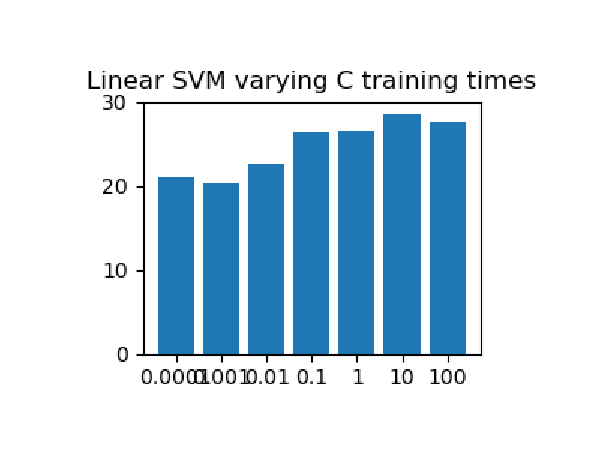
\includegraphics[width=5cm]{img/svm_3classclassifier_times_train_edit.eps}}
    \hfill
    \subfloat[Eval x:C y:Time(sec)]{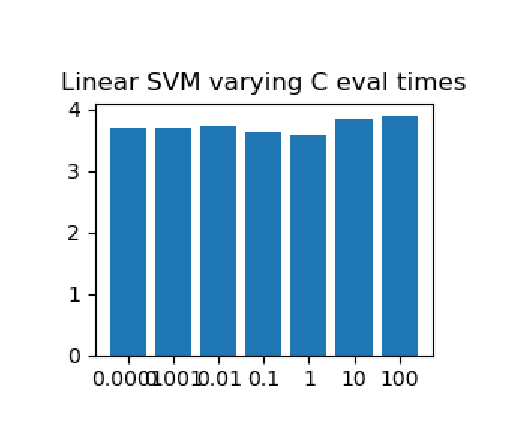
\includegraphics[width=5cm]{img/svm_3classclassifier_times_eval.eps}}\\
    \caption{Timings Linear}
\end{figure}
\subsection{\textit{RBF Kernel Models}}

\subsubsection{Accuracy over Gamma}
\begin{figure}[!htb]
    \centering
    \includegraphics[width=6cm]{img/svm_3classclassifier.png}
    \caption{x:Gamma Values y: Accuracies}
    \label{fig:my_label}
\end{figure}
\subsubsection{Training-Evaluation Times}
\subsubsection{Confusion Matrix-Heatmap}
\begin{figure}[!htb]
\centering
    \subfloat[Training x:Gamma Vals y:Time(sec)]{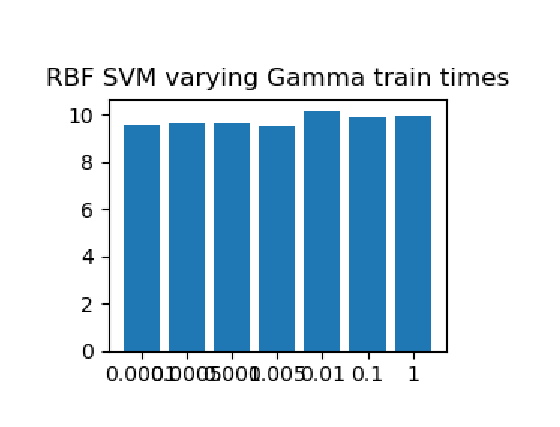
\includegraphics[width=5cm]{img/svm_3classclassifier_rbf_times_train.eps}}
    \hfill
    \subfloat[Eval x:Gamma Vals y:Time(sec)]{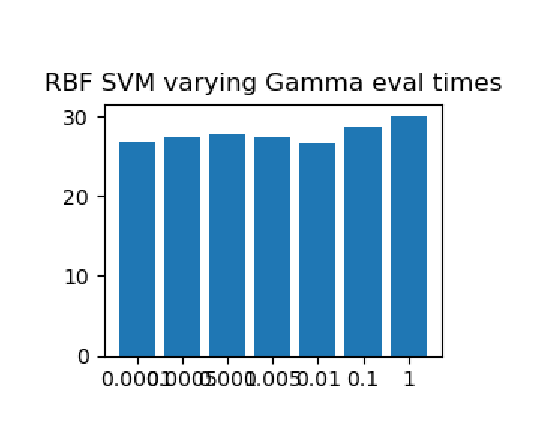
\includegraphics[width=5cm]{img/svm_3classclassifier_rbf_times_eval.eps}}\\
    \caption{Timings RBF}
\end{figure}

\subsection{Τελικά Σχόλια}
Παρατηρούμε ξεκάθαρο overfitting των μοντέλων και αδυναμία πρόβλεψης δειγμάτων στο test set σε σημεία που αναρωτιέμαι ότι κάτι έχει πάει λάθος στον κώδικα. Βέβαια το σύνολο δεδομένων ήταν πολύ μικρό και αυτό δικαιολογεί τα αποτελέσματα. Έτσι θα μπορούσα να χρησιμοποιήσω το \textit{LinearSVC} μοντέλο που έχει μεγαλύτερη ευελιξία σε πολλά δεδομένα και να πετύχω καλύτερα αποτελέσματα με μεγαλύτερο μέγεθος \textit{training} και \textit{test set}. Λόγω του μικρού συνόλου δεδομένων βλέπουμε και στο \textit{rbf }\textit{kernel} χειρότερα ακόμη αποτελέσματα κατά το τρέξιμο του κώδικα που είναι πιο εμφανείς οι τιμές των μετρικών. 

\end{document}